\documentclass[conference]{IEEEtran}
\IEEEoverridecommandlockouts
% The preceding line is only needed to identify funding in the first footnote. If that is unneeded, please comment it out.
\usepackage{url}
\usepackage{hyperref}
\usepackage{cite}
\usepackage{amsmath,amssymb,amsfonts}
\usepackage{algorithmic}
\usepackage{graphicx}
\usepackage{textcomp}
\usepackage{xcolor}
\usepackage{todo}
\usepackage{tikz}
\def\BibTeX{{\rm B\kern-.05em{\sc i\kern-.025em b}\kern-.08em
    T\kern-.1667em\lower.7ex\hbox{E}\kern-.125emX}}

\tikzstyle{block} = [rectangle, draw, 
    text width=5em, text centered, rounded corners, minimum height=2em]
\tikzstyle{oval} = [ellipse, draw, 
    text width=5em, text centered, rounded corners, minimum height=2em]
\tikzstyle{bt} = [rectangle, draw, 
    text width=1em, text centered, rounded corners, minimum height=2em]
\usetikzlibrary{calc}
\usetikzlibrary{arrows.meta}
\usetikzlibrary{positioning}
\usetikzlibrary{fit}
\usetikzlibrary{shapes.geometric}

\begin{document}

\title{VizAPI: Visualizing Interactions between Java Libraries and Clients
\thanks{This work was partially supported by Canada's Natural Science and Engineering Research Council.}
}

%\author{\IEEEauthorblockN{1\textsuperscript{st} Sruthi Venkatanarayanan}
%\IEEEauthorblockA{\textit{University of Waterloo} \\
%Waterloo, ON, CANADA \\
%s42venkat@uwaterloo.ca}
%\and
%\IEEEauthorblockN{2\textsuperscript{nd} Jens Dietrich
%\IEEEauthorblockA{\textit{Victoria University of Wellington}\\
%Wellington, NZ \\
%jens.dietrich@vuw.ac.nz}
%\and
%\IEEEauthorblockN{3\textsuperscript{rd} Craig Anslow}
%\IEEEauthorblockA{\textit{Victoria University of Wellington} \\
%Wellington, NZ\\
%craig.anslow@vuw.ac.nz}
%\and
%\IEEEauthorblockN{4\textsuperscript{th} Patrick Lam}
%\IEEEauthorblockA{\textit{University of Waterloo}\\
%Waterloo, ON, CANADA\\
%patrick.lam@uwaterloo.ca}
%}
%}


\author{\IEEEauthorblockN{Sruthi Venkatanarayanan, Patrick Lam}
\IEEEauthorblockA{University of Waterloo \\
Waterloo, ON, Canada \\
{\{s42venkat,patrick.lam\}@uwaterloo.ca}
\and
\IEEEauthorblockN{Jens Dietrich, Craig Anslow}
\IEEEauthorblockA{Victoria University of Wellington\\
Wellington, New Zealand \\
{\{jens.dietrich,craig.anslow\}@vuw.ac.nz}
}
}
}
\maketitle

\begin{abstract}
Software projects make use of libraries extensively. Libraries make available intended API surfaces—sets of exposed library interfaces that library developers expect clients to use. However, in practice, clients only use small fractions of intended API surfaces of libraries. We have implemented the VizAPI tool, which shows a visualization that includes both static and dynamic interactions between clients, the libraries they use, and  those libraries’ transitive dependencies (all written in Java). We then present some usage scenarios of VizAPI. One application, by client developers, is to answer a query about upstream code: will their code be affected by breaking changes in library APIs? Additionally, library developers can use VizAPI to find out about downstream code: which APIs in their source code are commonly used by clients? 
\end{abstract}

\begin{IEEEkeywords}
static program analysis,
dynamic program analysis,
API usage,
software evolution,
software maintenance
\end{IEEEkeywords}

\section{Introduction}
\section{Introduction}
\label{sec:introduction}

The long-term aspiration for software component reuse has finally arrived. This vision---of a component ecosystem enabling ubiquitous reuse and economies of scale---was first proposed over 50 years ago~\cite{mcilroy1968mass} and has finally become reality. Today's applications are largely built from existing components (with one major exception being embedded or safety-critical systems). A key contributor to this shift was the emergence of open source component repositories  such as Maven and npm: automated dependency resolution lowers the barriers for using third-party components, and developers can easily include components from them in their projects. The size and growth rate of these repositories is staggering.

However, there are still no silver bullets in software engineering~\cite{frederick87:_no_silver_bullet}. Component repositories are certainly not silver bullets, and their use comes with important trade-offs. The number of dependencies used by modern software has exploded, and so has their complexity~\cite{kikas2017structure,benelallam2019maven}: deeper, transitive dependencies are now common, components are upgraded more frequently, and developers increasingly struggle to deal with issues arising from those changes, such as: (1) dealing with conflicting versions of the same component (also known as dependency hell) and dealing with supply chain vulnerabilities of deep dependencies (often notified by bots creating pull requests); (2) new issues around security and resilience of the software supply chains, e.g. problems with changes to commodity components (as in the infamous left-pad incident~\cite{collins16:_how}) and novel attack patterns like typosquatting; and, (3) the use of unnecessary, bloated, and trivial dependencies~\cite{abdalkareem2017developers,soto2021comprehensive}.

So, components are revolutionary but bring new problems. Let's consider one problem: breaking changes. \textit{Potentially} breaking changes in library APIs are common~\cite{dietrich2014broken,raemaekers2014semantic}. However, any library change is only potentially breaking; does it \textit{actually} break any particular client? Only if a client uses a specific component API with an incompatible change.  

Yet, under plain Java (i.e. no runtime containers) and considering reflection, the API surface of any component is huge. Essentially: every method can be called, and every field can be read and written. Our research aims to answer the question: is the API surface huge in practice? Or, ought we better control component use? There are clear benefits in restricting the API surface: such restrictions can facilitate analyses that can calculate whether breaking changes are \textit{likely} to actually break clients.  Or, in terms of precision, added restrictions to the API surface would facilitate breakage analyses with fewer false positives (i.e., increased precision). 

As a second problem, consider the detection of vulnerabilities in dependencies. Detection is relatively straight-forward: compute the transitive closure of all dependencies, and cross-reference the transitive dependencies with vulnerability databases like CVEs. Tools like \textit{snyk} and \textit{dependabot} are based on this general idea. Some languages and build systems like npm have built-in language-specific support (\textit{npm audit}). The problem is again precision---listing something as a dependency does not mean that all of its functionality is used. So, if dependencies are sufficiently large and deep, a conservative approach inevitably results in false positives. Indeed, Elizalde Zapata et al~\cite{elizalde18:_towar_smoot_librar_migrat} found that 73\% of their studied clients with theoretically vulnerable dependencies were not actually at risk from CVEs in those dependencies, and Chinthanet et al~\cite{chinthanet20:_code_based_vulner_detec_node} implemented a code-based vulnerability detection tool for Node.js applications. Like the boy who cried wolf, false positives can lead to a potentially devastating impact on application security when true positives start being ignored, as demonstrated in the infamous Equifax incident~\cite{luszcz2018apache}. Sadowski et al~\cite{sadowski2018lessons}, among others, also cite the necessity for low false positive rates in developer tools.

The basic problem is well-known. In the history of Java (and other languages), several constructs enable component developers to better define and enforce the API surface, including access modifiers, modules, and bundles restricting access to packages, and packaging of components that only expose ``services'', i.e. instantiable classes implementing some abstract type that specifies the service. However, these restrictions always have to compete with the need to provide runtime introspection and code generation features.  Such features are needed to write generic software that can adapt to its usage context. A good example is the automated mapping of domain models to persistency (XML, JSON, RDMBMS, etc).

%  This is often part of another successful trend in modern software engineering---convention over configuration---where services are inferred based on implicit interfaces defined by conventions. 

%In a sense, this has created an arms race:  technologies trying to control APIs versus techniques allowing software to bypass restrictions. This is the space that developers have to navigate when writing modern software.

This paper aims to take a snapshot of where current software practices stand: we investigate how APIs are used and misused. 
We intend to make our code and data available with the camera-ready version of this paper.

Our contributions include:
\begin{itemize}
\item a classification of API uses and mis-uses along four dimensions (Section~\ref{sec:classification}), with examples (Section~\ref{sec:api-usage-examples});
\item a tool to instrument Java code and collect dynamic instrumentation data about API uses in practice (Section~\ref{sec:technique});
\item an empirical study (Section~\ref{sec:results}) to investigate a collection of 11 libraries and 38 clients: (1) API mis-uses exercised during client tests; (2) sizes and overlaps of the API surfaces of the libraries used by the client test suites.
\end{itemize}

%To expand on our aims, we aim to characterize (1) API uses of libraries that are not anticipated by the library developers (``mis-uses'') as well as (2) the empirical extent of API uses by their clients (``API surfaces''). 

{\bf Findings.} Our results indicate that API mis-uses are generally rare: developers respect modularity declarations and seldom use reflection to bypass access modifiers (with serialization as a key exception). On the other hand, clients use widely varying portions of their libraries.

Actionable outcomes, which we discuss in Section~\ref{sec:discussion}, include guidance to API designers, based on the fact that API usages are sparse, as well as suggestions for tool designers.


\section{Related Work}
\label{sec:related-work}
A representative tool from the software visualization literature is
CodeSurveyor, by Hawes et al~\cite{hawes15:_codes}, which visualizes large
codebases using the analogy of cartographic maps. While it
incorporates dependency information into the layout of the map, VizAPI
differs from CodeSurveyor in that VizAPI focusses on usage relationships
between different modules (e.g. API invocations) using test
cases and static analysis to identify relationships between clients and libraries, rather
than investigating a particular system, as CodeSurveyor does.  Earlier
work includes the software cartography project by Kuhn et
al~\cite{kuhn10:_softw} and software terrain maps by DeLine~\cite{deline05:_stayin}.

% could mention
%software visualization/history animation:

%Gource
%code_swarm https://effectivesoftwaredesign.com/2012/05/24/code-swarm-visualizing-the-evolution-of-software-systems/

%% There is a large body of work investigating API usages, particularly
%% in mining API specifications, as first introduced by Ammons et
%% al~\cite{AmmonsETAL02MiningSpecifications}. 
%% Saied et
%% al~\cite{saied15:_minin_multi_api_usage_patter} studied which API
%% calls tended to co-occur in client code and inferred co-usage
%% relationships between these calls. Like them, we are specifically not
%% investigating sequencing relationships between API calls.

Hejderup and Gousios~\cite{DBLP:journals/jss/HejderupG22} explore a
question which is central to our approach---how well do client tests
exercise their dependencies' libraries? The dynamic part of our approach relies on
client test suites exercising enough of the dependencies to get valid
dynamic results from our analyses. They conclude that a combination of
static and dynamic analysis of the client has some chance of detecting
breaking changes in its dependencies, and we accordingly use static
analysis to supplement our dynamic results.

%% Thummalapenta and Xie~\cite{thummalapenta08:_spotw} presented
%% SpotWeb, which identifies framework hotspots (often-used APIs) and coldspots (never-used APIs).
%% Their notion of API
%% usage is similar to ours, but they perform a static search to identify
%% uses, while we additionally dynamically observe test executions. They
%% also identify the top $N$ percent of used APIs as hotspots, and unused
%% APIs as
%% coldspots. Viljamaa~\cite{viljamaa03:_rever_engin_framew_reuse_inter}
%% also identified hotspots, via concept analysis.

Call graph visualization is, of course, a well-known technique, as seen e.g. by the Reacher tool~\cite{latoza11:_visual_call_graph}. 
VizAPI also presents static and dynamic call information. However, we designed
it to support decisions about library/client interactions: the granularity of nodes is packages (typically it is methods);
and the layout is influenced by frequency of interactions.

Our overall goal is to help both client and library developers understand
client uses of library code. Clients benefit from sharpened warnings
about unsafe upgrades, knowledge that some upgrades are safe, and
having reduced attack surfaces. Library upgrades have been
investigated by many researchers, including Lam et
al~\cite{lam20:_puttin_seman_seman_version} and Kula et al~\cite{kula18:_do_devel_updat_their_librar_depen}. Kula et al found that most
software had outdated dependencies, and that software developers disliked being required to constantly upgrade their
libraries. Kula et al~\cite{kula14:_visual_evolut_system_their_librar_depen} also developed a tool
to visualize changes in dependencies over time---but not how a particular client depends on its libraries. 
Our VizAPI tool's dependency visualizations will help developers
prioritize required upgrades as low-effort or high-effort.
Foo et al~\cite{foo18:_effic_static_check_librar_updat}
proposed a static analysis which detected safe upgrades, but could
only certify safety for 10\% of upgrades; our combined static and
dynamic approach presents the developer with more information and
enables more upgrades. 

Bergel et al~\cite{bergel14:_domain_specif_languag_visual_softw_depen_graph} propose the {\sc Graph} DSL
for software visualizations. That language could generate static representations similar to VizAPI's; however,
VizAPI chooses a specific point in the design space, and we argue that this point is useful for helping developers understand
potential impacts of upgrades.


\section{VizAPI}
\label{sec:viz-api}

\begin{figure*}[h]
\begin{center}
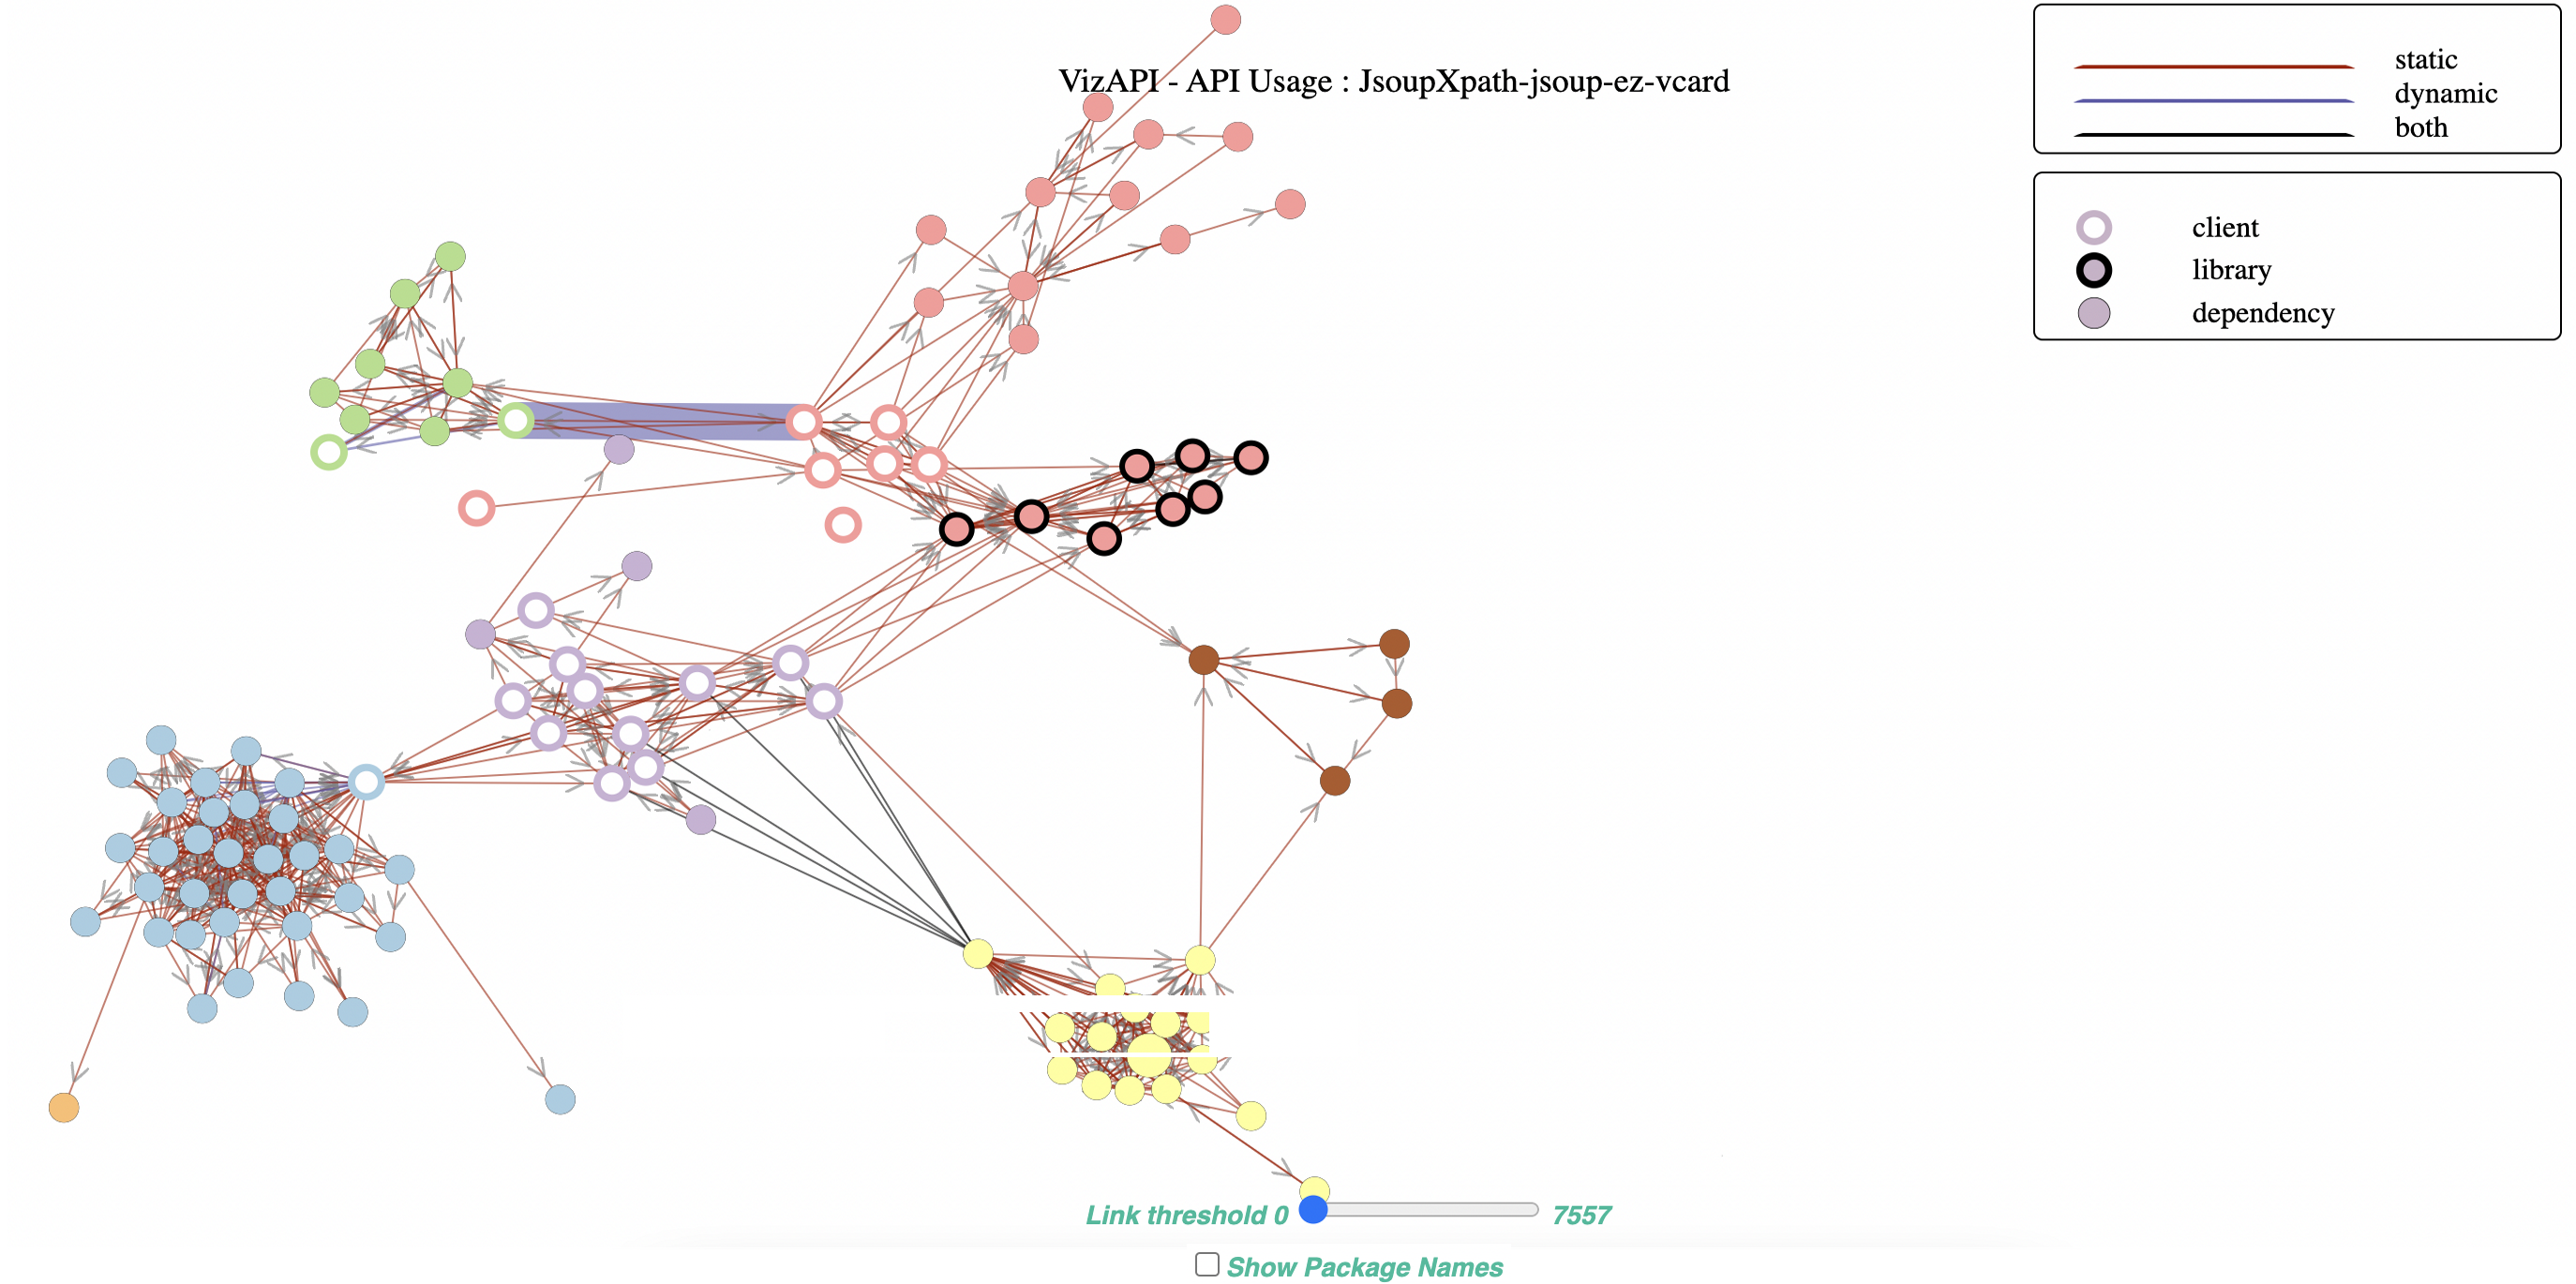
\includegraphics[scale=1,width=15cm,height=8cm]{images/usage-scenario1.png}
\caption{Usage Scenario 1: jsoup (library), JsoupXpath (client), ez-vcard (client)}
\label{fig:usagescenario1}
\end{center}
\end{figure*}

\subsection{Design}
\label{sec:collecting-data}
Our goal is to visualize interactions between different software components---between
clients and libraries, and between libraries and other libraries. We now explain
how we collect static and dynamic information about software behaviour.

\paragraph{Static information} ???

\paragraph{Dynamic information} We collect dynamic data by running client
test suites under instrumentation. 
The instrumentation records API
uses which cross client/library boundaries, as well as library/library boundaries
for libraries that are transitively used. We use
Javassist~\cite{chiba00:_load_struc_reflec_java} to perform the
instrumentation and then the build system of each project (Maven or Gradle) to run its
tests. Figure~\ref{fig:workflow} summarizes our instrumentation and
data capture workflow. We next describe our instrumentation implementation in detail.

We identify interactions across the client/library boundaries by
inspecting JAR files of each software component to obtain a list of
classes for every component. We associate classes and their members to
components based on these lists. \todo{is this still true?}

\begin{figure*}[h]
 \begin{center}
\resizebox{0.7\textwidth}{!}{
  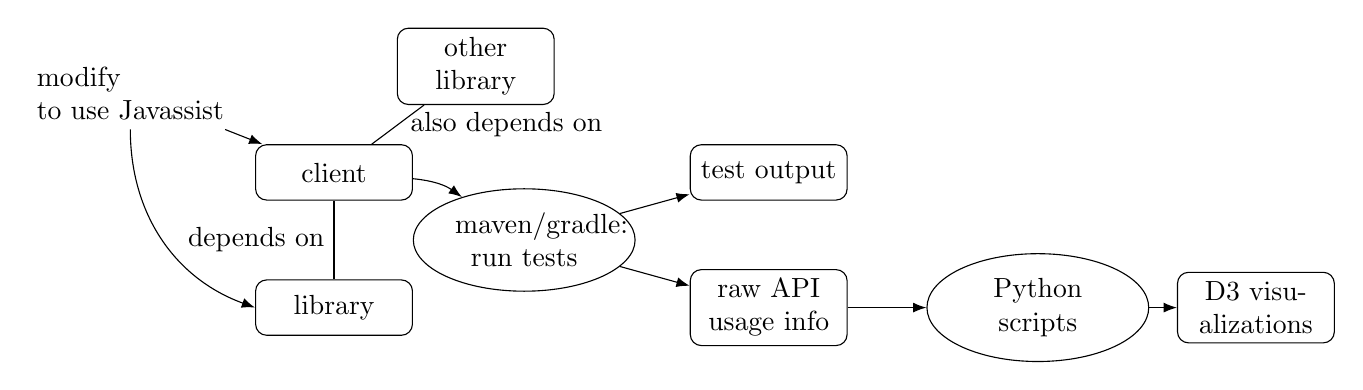
\begin{tikzpicture}
    \node[block] (client) {client};
    \node[block,below=1cm of client] (library) {library};

    \draw (library) -- node[left] (depends) {depends on} (client);

    \node[above left=.75em of client] (ja) {\begin{minipage}{7em} modify \\to use Javassist \end{minipage}};
    \draw[-Latex] (ja) -> (client);
    \draw[-Latex] (ja) to [->,bend right=35] (library.west);

    \node[block, above right=2em of client,xshift=-2em] (olib) {other library};
    \draw (client) -- node[right,xshift=.1em] (also) {also depends on} (olib);

    \node[oval,right=of depends] (test) {maven/gradle: run tests};

    \draw[-Latex] (client) to [->,bend left=15] (test);

    \node[block, right=10em of client] (output) {test output};
    \node[block, right=10em of library] (raw) {raw API usage info};

    \draw[-Latex] (test) to (output);
    \draw[-Latex] (test) to (raw);

    \node[oval, right=of raw] (Py) {Python scripts};
    \draw[-Latex] (raw) to (Py);

    \node[block, right=1em of Py] (viz) {D3 visualizations};
    \draw[-Latex] (Py) to (viz);
  \end{tikzpicture}
}
  \caption{Our instrumentation workflow. We modify existing project infrastructure to instrument clients and to run their test suites, producing raw data, which we process with our Python scripts to create D2 visualizations.}
  \label{fig:workflow}
 \end{center}
\end{figure*}


At every invoke instruction in every
loaded method which transfers control between the client and the
library, we add code to record that invoke by incrementing a counter.
We handle both static and virtual (including special, virtual,
interface, and dynamic) calls. Crossing the client/library boundary
includes callbacks from the library to the client as well as the conventional
calls from the client to the library. 

We also record field accesses (direct and reflective), dynamic proxies
and reflective calls, Java annotations, implementations,
instantiations, and casts.


\subsection{Visualization System}
\label{sec:vis-system}

Once we have generated data, we separate all the different interactions
into two categories---static and dynamic. We then use a modified version
of the d3graph \todo{cite} library in Python to generate a d3js \todo {cite} 
visualization. We now briefly describe the graphs generated by VizAPI.
The graphs are force-directed based on edge weights, which are the
frequency of interactions between the source and target nodes.
Each node is a set of one or more packages(or classes or methods) 
that belong to the same jar. Nodes are coalesced if they belong to the same 
jar and have the same incoming and outgoing edges. Each edge is directed 
from the source package(s) to the target package(s) and represents an interaction 
(invocations, fields, annotations, subtyping) between packages. We run a 
clustering algorithm and colour nodes based on the cluster 
(could comprise same or different jars) that they belong to. 
Hovering on a node shows you the list of packages and 
the jar they belong to, 
formatted as “jar : $<$space separated list of packages$>$”.


\subsection{Case Study}
\label{sec:evaluation}

We conducted a pilot study of VizAPI on an 85-project subset of the
Duets benchmarks~\cite{durieux21}. Our study included 10 libraries and
their clients. For libraries, we pick the most popular Maven repositories 
in different categories such as logging and json parsing. We pick clients partly
from popular Github repositories and partly from Duets~\cite{durieux21}.
We collect both static and dynamic data for these projects.

\begin{figure*}[h]
\begin{center}
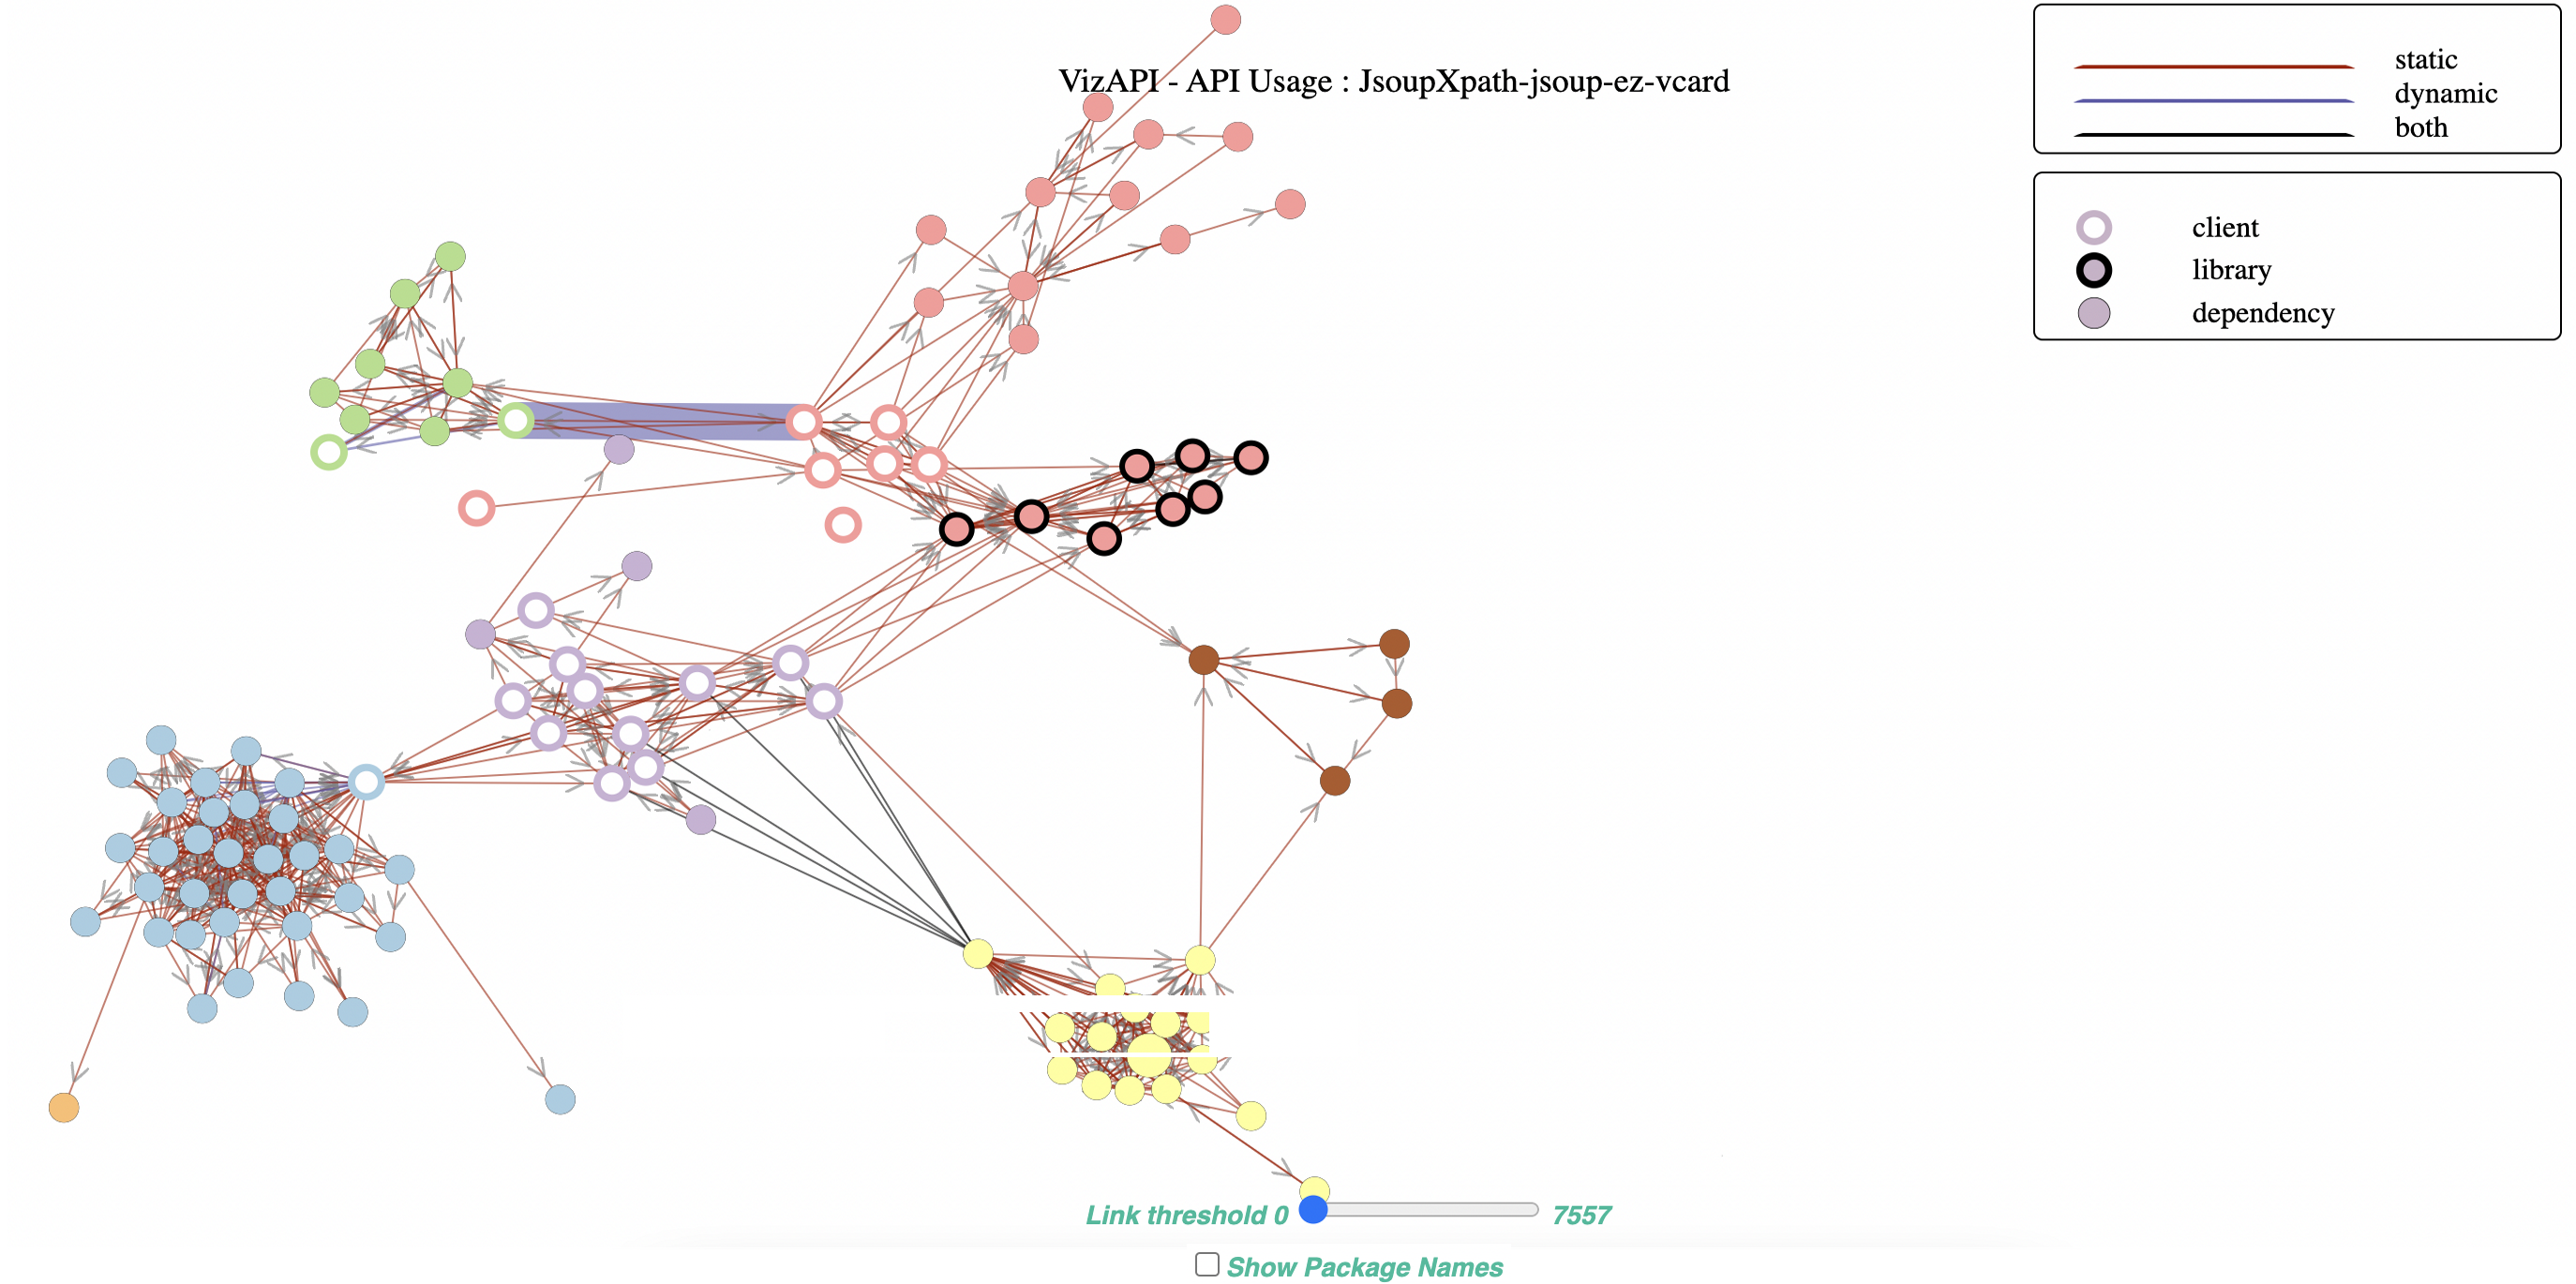
\includegraphics[scale=1,width=18cm,height=8cm]{images/usage-scenario1.png}
\caption{Usage Scenario 1: jsoup (library), JsoupXpath (client), ez-vcard (client)}
\label{fig:usagescenario1}
\end{center}
\end{figure*}

Now, we walk through an example usage scenario of VizAPI.
The graph in Figure~\ref{fig:usagescenario1} represents static and dynamic interactions of 2 clients with the jsoup\footnote{\url{https://github.com/jhy/jsoup}\label{jsoup}} library. Our clients are JsoupXpath\footnote{\url{https://github.com/zhegexiaohuozi/JsoupXpath}\label{jsoupxpath}} and ez-vcard\footnote{\url{https://github.com/mangstadt/ez-vcard}\label{ez-vcard}}.

We can start our exploration with the cluster of pink nodes. Many of these nodes belong to either JsoupXpath or jsoup. When we hover over them, the hover hints tell us that the client JsoupXpath calls directly into \texttt{org.jsoup.nodes} and \texttt{org.jsoup.select}. Notably, and as we might expect, we can see that \texttt{org.jsoup.helper} and \texttt{org.jsoup.internal} aren't called directly by JsoupXpath. This would mean that breaking changes in \texttt{org.jsoup.helper} or \texttt{org.jsoup.internal} wouldn't directly affect JsoupXpath\footnote{As a specific example, the retraction of an internal jsoup API would not break this client. Behavioural changes that are directly passed through to the external API, e.g. through delegation, can still break clients, but we can consider those to be changes in the external API.} Similarly, ez-vcard directly calls into \texttt{org.jsoup}.

ez-vcard also calls into jackson-core\footnote{\url{https://github.com/FasterXML/jackson-core}\label{jackson-core}} and jackson-databind\footnote{\url{https://github.com/FasterXML/jackson-databind}\label{jackson-databind}}, which are very tightly coupled amongst their own packages and with each other. This could mean that breaking changes in these libraries can propagate to many of their own packages.
.



\section{Discussion}
\label{sec:discussion}

CHA brings in a lot of stuff


\bibliographystyle{plainurl}
\bibliography{bibliography}

\end{document}
